%!TEX root = ../thesis.tex
%*******************************************************************************
%*********************************** Methods *****************************
%*******************************************************************************

\chapter{Statistical methods for survival data}\label{cha:methods}

\graphicspath{{01_Introduction/Figs/}}

This chapter provides an introduction to the statistical methods used throughout the thesis, beginning with a description of survival data and of two classical survival methods:\ the Kaplan-Meier estimator and Cox proportional hazards model. I explain how the presence of competing risks can be a challenge for these classical methods, and describe two analogous survival methods which can account for competing risks. These competing risks methods are generalised to multi-state survival models through the theory of counting processes.

Following this is an introduction to key concepts in causal inference and a description of study designs used for observational data collection, with examples of common biases seen in these data.

\section{Survival analysis}

Survival analysis involves the analysis of time-to-event data, also termed `survival data', where the event could be any outcome of interest, and the time refers to the duration from a given origin to the occurrence of an event (the endpoint)~\parencite{Collett2023-bg}.

This section introduces survival data in the context of infectious disease studies and outlines methods to account for data censoring and truncation.

\subsection{Overview of survival data}

In studies of infectious disease, survival data are often used to describe clinical origins and endpoints, for example:\ from study recruitment to the time of infection; from hospitalisation to discharge; or from infection to death. These data may be combined with information on patient characteristics, such as age, gender, or socioeconomic status, and clinical variables, such as uptake of vaccination, or initiation of treatment~\parencite{Collett2023-bg}.

\subsection{Censoring and truncation}\label{sec:censoring-truncation}

Two common features of survival data are censoring and truncation. These arise due to incomplete or non-observation of time-to-event information and may take a number of forms.

\subsubsection{Censoring}

Censoring in survival data occurs when information about an individual is only known within certain intervals, or `censoring times', $(C_l, C_r)$~\parencite{Klein2005-ls}. Various categories of censoring exist, which lead to different specifications of the likelihood function (discussed further in Section~\ref{sec:likelihood}).

\textbf{Right-censoring} is when we lack information to the `right' (or future) of the right-censoring time $C_r$. For example, if study follow-up finishes before the event of interest, $X$, has taken place for an individual, this individual is right-censored at time $C_r < X$~\parencite{Klein2005-ls}.

\textbf{Left-censoring}, on the other hand, is when the event of interest, $X$, has occurred at an unknown point before the left-censoring time, $C_l$, e.g.\ if the event of interest occurs before the person is first observed in the study, this individual is left-censored at time $C_l > X$~\parencite{Collett2023-bg}.

Censoring may also be intentionally imposed on a dataset, termed \textbf{administrative censoring}. Administrative censoring may be used to limit the time-to-event data for each individual to a pre-specified cut-off, with any events beyond this period not considered, e.g.\ mortality within 30 days of hospital admission~\parencite{Collett2023-bg}. Examples of right-censoring, left-censoring, and administrative censoring in a patient-level time-to-event dataset are shown in Figure~\ref{fig:censoring}.

\begin{figure}[!ht]
    \centering
    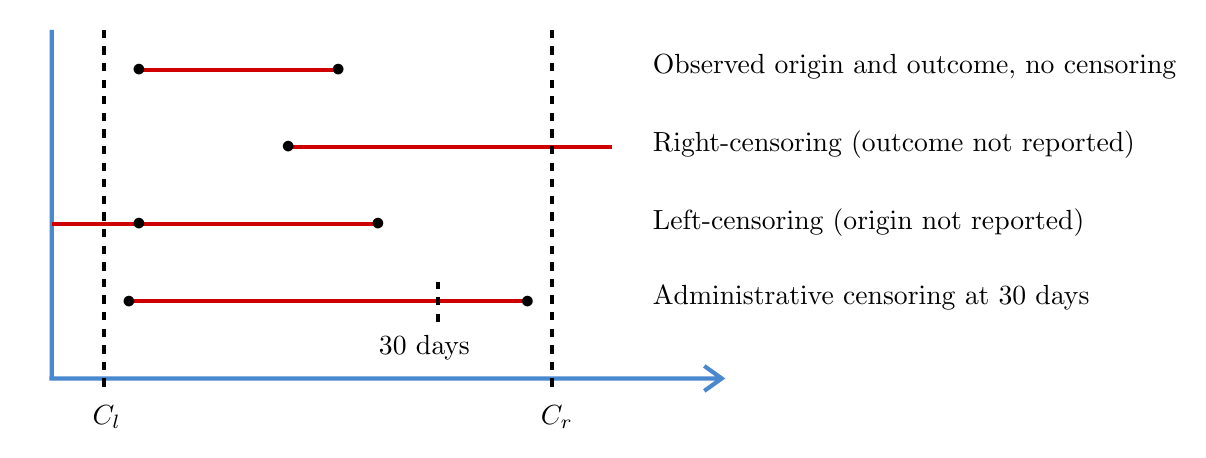
\begin{tikzpicture}[x=0.9pt,y=0.9pt,yscale=-1,xscale=1]
        \path (70,230); %set diagram left start at 0, and has height of 200

        %Shape: Axis 2D [id:dp048941842347560494] 
        \draw [color={rgb, 255:red, 73; green, 135; blue, 206 }, draw opacity=1 ][line width=1.5][-]
        % axes
        (78.67,210.33) -- (348.67,210.33)
        (79.67,70.33) -- (79.67,210.33)

        % arrow
        (341.67,205.33) -- (348.67,210.33) -- (341.67,215.33);

        \draw;

        \draw [color={rgb, 255:red, 206; green, 0; blue, 0 }, draw opacity=1][line width=1.5][-]

        (110.67,179.33) -- (270.67,179.33)
        (79.67,148.33) -- (210.67,148.33)
        (174.67,117.33) -- (304.67,117.33)
        (114.67,86.33) -- (194.67,86.33);

        \draw;

        \draw [color={rgb, 255:red, 0; green, 0; blue, 0 }, draw opacity=1][line width=1.5][-][dashed]
        (280.67,70.33) -- (280.67,215.33)
        (100.67,70.33) -- (100.67,215.33)
        (234.67,187.66) -- (234.67,171.66);
        \draw;

        \draw [-] (95,220) node [anchor=north west][inner sep=0.75pt] [align=left] {$C_l$};
        \draw [-] (275,220) node [anchor=north west][inner sep=0.75pt] [align=left] {$C_r$};

        \draw [-] (320,79) node [anchor=north west][inner sep=0.75pt] [align=left] {Observed origin and outcome, no censoring};
        \draw [-] (320,110) node [anchor=north west][inner sep=0.75pt] [align=left] {Right-censoring (outcome not reported)};
        \draw [-] (320,141) node [anchor=north west][inner sep=0.75pt] [align=left] {Left-censoring (origin not reported)};
        \draw [-] (320,172) node [anchor=north west][inner sep=0.75pt] [align=left] {Administrative censoring at 30 days};

        \draw [-] (210,192) node [anchor=north west][inner sep=0.75pt] [align=left] {30 days};

        % dots
        \foreach \Point in {
                (110.67,179.66),
                (270.67,179.66),
                (174.67,117.66),
                (114.67,148.66),
                (210.67,148.66),
                (114.67,86.66),
                (194.67,86.66)}{
                \node at \Point {$\bullet$};
            }

    \end{tikzpicture}
    \caption[Examples of right, left, and administrative censoring for patients in time-to-event data with origin and outcome information reported]{Examples of right, left, and administrative censoring for patients in time-to-event data with origin and outcome information reported. $C_l$: left-censoring time, $C_r$: right-censoring time, $\bullet$: reported origin, outcome, or intermediate event.}\label{fig:censoring}
\end{figure}

A more general form of censoring is \textbf{interval-censoring}, which occurs when the event of interest, $X$, takes place in-between measurements, i.e.\ within a censoring interval $(L, R]$, $L < X < R$. An example is the infection time for an individual --- typically not directly observed, but known to occur in-between a negative and positive test. Interval censoring is a feature of `intermittently-observed' data, where individuals are tested for the presence of infection at several time-points, and can be used to detect changes in an individual's infection status when testing is sufficiently frequent~\parencite{van-den-Hout2016-xy, Klein2005-ls}, as shown in Figure~\ref{fig:intermittent-data}.

\input{01_Introduction/Figs/intermittent-observed}

\subsubsection{Truncation}

A second common feature of survival data is truncation. Truncation is related to censoring, although whereas with censored data there is at least partial information about an individual, with truncated data information outside of the truncation interval $(Y_l, Y_r)$ is not observed at all~\parencite{Klein2005-ls}. As with censoring, both left, right, and interval-truncation are possible.

\textbf{Left-truncation} occurs when only event-times which take place after the left-truncation time, $Y_l$, are available, e.g.\ if individuals whose event of interest takes place prior to the study, $X < Y_l$, are not recorded, they are left-truncated.

\textbf{Right-truncation} occurs when only event-times which take place before the right-truncation time, $Y_r$, are available, e.g.\ if records are only submitted once an outcome has taken place, with no knowledge of individuals at risk but whose event of interest occurs after the study endpoint, $X > Y_r$, these individuals are right-truncated~\parencite{Klein2005-ls}. Examples of left and right-truncated patient-level time-to-event data are shown in Figure~\ref{fig:truncation}.

\begin{figure}[!ht]
    \centering
    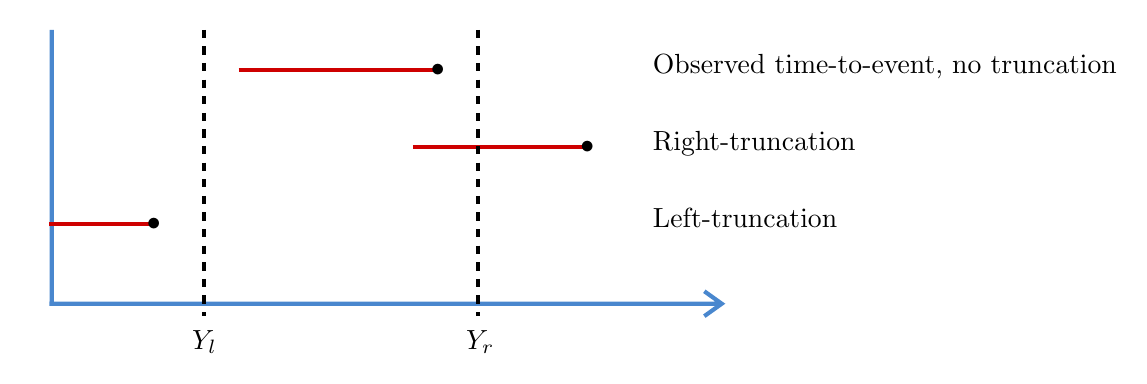
\begin{tikzpicture}[x=0.9pt,y=0.9pt,yscale=-1,xscale=1]
        \path (70,200); %set diagram left start at 0, and has height of 200

        %Shape: Axis 2D [id:dp048941842347560494] 
        \draw [color={rgb, 255:red, 73; green, 135; blue, 206 }, draw opacity=1 ][line width=1.5][-]
        % axes
        (78.67,180.33) -- (348.67,180.33)
        (79.67,70.33) -- (79.67,180.33)

        % arrow
        (341.67,175.33) -- (348.67,180.33) -- (341.67,185.33);

        \draw;

        \draw [color={rgb, 255:red, 206; green, 0; blue, 0 }, draw opacity=1][line width=1.5][-]

        (78.67,148.33) -- (120.67,148.33)
        (224.67,117.33) -- (294.67,117.33)
        (154.67,86.33) -- (234.67,86.33);

        \draw;

        \draw [color={rgb, 255:red, 0; green, 0; blue, 0 }, draw opacity=1][line width=1.5][-][dashed]
        % reporting date
        (250.67,70.33) -- (250.67,185.33)
        (140.67,70.33) -- (140.67,185.33);
        \draw;

        \draw [-] (135,190) node [anchor=north west][inner sep=0.75pt] [align=left] {$Y_l$};
        \draw [-] (245,190) node [anchor=north west][inner sep=0.75pt] [align=left] {$Y_r$};

        \draw [-] (320,79) node [anchor=north west][inner sep=0.75pt] [align=left] {Observed time-to-event, no truncation};
        \draw [-] (320,110) node [anchor=north west][inner sep=0.75pt] [align=left] {Right-truncation};
        \draw [-] (320,141) node [anchor=north west][inner sep=0.75pt] [align=left] {Left-truncation};

        % dots
        \foreach \Point in {
                (120.67,148.66),
                (294.67,117.66),
                (234.67,86.66)}{
                \node at \Point {$\bullet$};
            }

    \end{tikzpicture}
    \caption[Examples of left and right-truncation for patients in time-to-event data]{Examples of left and right-truncation for patients in time-to-event data, assuming only information within the truncation interval $(Y_l, Y_r)$ is observed. $Y_l$: left-truncation time, $Y_r$: right-truncation time, $\bullet$: outcome time.}\label{fig:truncation}
\end{figure}

\subsection{Cumulative incidence, survivor, and hazard functions}

Because censored and truncated survival data are not fully observed, estimating a distribution for the time-to-event presents a challenge for standard statistical methods. For valid statistical estimation of these data, a specific class of survival methods have been developed which can account for different types of censoring and truncation.

These methods are based on the concept of the \textit{survivor function}, which describes the probability of surviving beyond a given time, and the \textit{hazard function}, which describes the instantaneous rate of failure at time $t$, given survival up until time $t$~\parencite{Collett2023-bg}.

\subsubsection{Cumulative incidence function}

Let $T$ be the independent and identically distributed (i.i.d)\nomenclature[z]{i.i.d.}{Independent and identically distributed} random variable representing the survival time, $T = t>0$, for an individual, and assume this random variable has a probability distribution with probability density function $f(t)$.

The distribution function of $T$, also known as the cumulative incidence function, is the probability of `failure' before time $t$, defined as~\parencite{Collett2023-bg}:
%
\[
    F(t) = \Pr(T<t) = \int_0^t f(u) \dif u
\]

\subsubsection{Survivor function}

The survivor function is the probability of surviving past time $t$, defined as:
%
\[
    S(t) = \Pr(T \geq t) = 1-F(t)
\]

\subsubsection{Hazard function}

The hazard function is the instantaneous rate of failure at time $t$, given survival up until time $t$, defined as:

\begin{equation}
    h(t) = \lim_{\delta t \downarrow 0} \left\{\frac{\Pr(t \leq T < t + \delta t \mid T \geq t)}{\delta t}\right\}
    \label{eq:hazard-function}
\end{equation}

By conditional probability, $\Pr(A \mid B) = \Pr(AB)/\Pr(B)$, so the hazard function can also be expressed as:
%
\begin{align*}
    h(t) & = \lim_{\delta t \downarrow 0} \left\{\frac{\Pr(t \leq T <t + \delta t)}{\delta t \Pr(T \geq t)}\right\} \\
         & = \lim_{\delta t \downarrow 0} \left\{\frac{F(t + \delta t) - F(t)}{\delta t S(t)}\right\}               \\
         & = \lim_{\delta t \downarrow 0} \left\{\frac{F(t + \delta t) - F(t)}{\delta t}\right\}\frac{1}{S(t)}
\end{align*}

This limit is the definition of the derivative of $F(t)$ with respect to $t$, and therefore equal to $f(t)$~\parencite{Collett2023-bg}:
%
\[
    \lim_{\delta t \downarrow 0} \left\{\frac{F(t + \delta t) - F(t)}{\delta t}\right\} = \frac{\dif}{\dif t}F(t) = f(t)
\]

hence the hazard function can be re-written:
%
\begin{equation}
    h(t) = \frac{f(t)}{S(t)}
    \label{eq:hazard-survivor}
\end{equation}

% from which the \textit{cumulative hazard function} may be defined~\parencite{Collett2023-bg}:
% %
% \[
%     H(t) = \int_0^t{h(u) \dif u}
% \]

\section{Statistical inference in survival analysis}

Statistical inference is the process of using data to infer the properties of an underlying probability distribution. In this section I describe the `likelihood function', used to connect statistical models to observed data in the frequentist and Bayesian frameworks. Two classical methods of statistical inference for survival analysis data are shown:\ the Kaplan-Meier estimator and Cox proportional hazards model. These methods are well-suited to studies of simple disease processes, for example when we are only interested in the effect of an intervention on a final outcome, irrespective of any intermediate events~\parencite{Austin2017-im}.

\subsection{Likelihood estimation}

\subsubsection{Frequentist and Bayesian likelihood}

The likelihood function, $L$, is used to link statistical models to observed data. The likelihood is the probability of observing the data, $D$, given the parameters, $\theta$, of the model and formally expressed as:
%
\[
    L(\theta \mid D) = f(D \mid \theta) = \prod_i f(X_i \mid \theta)
\]

where $f$ is the probability density function, and $X_i$ are assumed to be i.i.d observations in the data~\parencite{Wasserman2004-gw}.

In the `frequentist' framework the parameters of a statistical model are considered to have a fixed `true' unknown value to be estimated, and the data are realisations of random variables. The parameters of the model are estimated by maximising the likelihood to obtain the \textit{maximum likelihood estimate} (MLE)\nomenclature[z]{MLE}{Maximum likelihood estimate}, denoted $\hat{\theta}$~\parencite{Wasserman2004-gw}.

Bayesian methods are an alternative to maximum likelihood estimation, used to estimate the probability distribution of the parameters of the model given the data, known as the `posterior distribution'. In the Bayesian framework, all quantities (both observable quantities and parameters) are considered as random variables, with observed data being realisations of these random variables. The posterior distribution, $f(\theta \mid D)$, is related to the likelihood function, $f(D \mid \theta)$, via Bayes formula~\parencite{Wasserman2004-gw}:
%
\[
    f(\theta \mid D) = \frac{f(D \mid \theta)f(\theta)}{f(D)}
\]

\subsubsection{Likelihoods for censored and truncated data}\label{sec:likelihood}

Constructing likelihoods for censored or truncated data requires careful consideration of the information provided by each observation. The likelihood components provided by censored observations are described by~\cite{Klein2005-ls}:
%
\begin{itemize}
    \item for exactly observed data:\ information on the probability of the event occurring at this time, i.e.\ $f(X)$;
    \item for right-censored observations:\ information on the survivor function up to a certain time, i.e.\ $S(C_r)$;
    \item for left-censored observations:\ information on the cumulative incidence up to a certain time, i.e.\ $F(C_l)$;
    \item for interval-censored observations:\ information on the probability that the event is within this interval, i.e.\ $S(L) - S(R)$.
\end{itemize}

As data may be observed with different levels of censoring or truncation, the likelihood function is constructed from the joint product of each component for each observation $i$:
%
\[
    L \propto \prod_{i} f(X_i) \prod_{i} S(C_{r,i}) \prod_{i} F(C_{l,i}) \prod_i (S(L_i) - S(R_i))
\]

The equivalent likelihood components for truncated data provide information on conditional probabilities of events, i.e.\ $f(X)/F(Y_r)$ for right-truncated observations, where observation is conditional on the event of interest having occurred by truncation time $Y_r$~\parencite{Klein2005-ls}.

\subsection{Parametric and non-parametric models}

The statistical models used for estimating model parameters may be parametric or non-parametric. In general, parametric models rely on assumptions about the distribution of the underlying survival times, so careful selection of this distribution is needed for valid inference.

In contrast, non-parametric models require fewer assumptions about the survival distribution, so can be applied when the functional form of the model is not known, but may require more data and not allow for extrapolation beyond the time period of the observed data. Comparisons to non-parametric estimates can be made to assess the fit of a parametric model~\parencite{Aalen2008-rf,Jackson2022-lt}.

\subsection{Kaplan-Meier estimator}

The Kaplan-Meier estimator is a widely-used, non-parametric method to estimate the survivor function from censored data, and defined as:
%
\begin{equation}
    \hat{S}(t) = \prod_{t_k \leq t}\left(\frac{n_k - d_k}{n_k}\right)
    \label{eq:kaplan-meier}
\end{equation}

where $d_k$ is the number of events, and $n_k$ is the number of individuals at risk at time $t_k \leq t$~\parencite{Collett2023-bg}.

\subsection{Cox proportional hazards model}\label{sec:cox-model}

The Cox proportional hazards model is used to relate survival times to explanatory variables via regression. The model is `semi-parametric', as the baseline hazard is estimated non-parametrically while the effects of covariates are estimated parametrically~\parencite{Cox1972-ww}. The Cox proportional hazards model assumes that the hazard of death at any given time for an individual in one group is \textit{proportional} to the hazard of death at the same time for an individual in a different group. This is expressed by writing the hazard function conditional on a given set of $m$ constant or time-varying covariates $\bm{z} = \{z_{1}\ldots, z_{m}\}$ as:
%
\[
    h(t \mid \bm{z}) = h^{(0)}(t)\exp\left(\sum_{m=1}^{M}\beta_{m}z_{m}\right) \equiv h^{(0)}(t)\exp(\bm{\beta}^\mathsf{T}\bm{z})
\]

where $h^{(0)}(t)$ is the baseline hazard function, and $\beta_{m}$ are the regression coefficients. Notably that the `hazard ratio' for the $m$th covariate is a constant~\parencite{Klein2005-ls}:
%
\[
    \frac{h(t \mid z_m = 1)}{h(t \mid z_m = 0)} = \frac{h^{(0)}(t)\exp(\beta_m 1)}{h^{(0)}(t)\exp(\beta_m 0)} = \exp(\beta_{m})
\]

The regression coefficients $\beta_{m}$ are estimated by maximising the partial likelihood $L(\bm{\beta})$:
%
\[
    L(\bm{\beta}) = \prod_{i \in D}\frac{\exp(\bm{\beta}^\mathsf{T}\bm{z}_{d_i})}{\sum_{j \in R_i}\exp(\bm{\beta}^\mathsf{T}\bm{z}_j)}
\]

where $D = \{T_1, T_2, \ldots, T_n\}$ are the set of distinct failure times, $R_i$ is the set of all individuals who are at risk of failure immediately before time $T_i$, $\bm{z}_{d_i}$ is the covariate vector for an individual who failed at time $T_i$, and $\bm{z}_j$ is the covariate vector for the $j$th individual at risk at time $T_i$~\parencite{Klein2005-ls}.

Further details of the Cox proportional hazards model, specifically of how to account for non-proportional hazards and correlation in survival times, are included in Appendix~\ref{appx:methods}.

\section{Competing risks survival models}\label{sec:cr-models}

In medical cohort studies, multiple end-points (e.g.\ death, intensive care admission, and discharge) may be considered. These multiple end-points are known as \textit{competing risks} and may hinder the event of interest, or modify the chance that this event occurs~\parencite{Collett2023-bg}. Kaplan-Meier and Cox proportional hazards models treat competing risks as censored observations, and do not account for dependencies between events. Hence the assumption of independent times-to-events in these conventional survival analyses is violated in the presence of competing risks~\parencite{Andersen2012-gp, Putter2007-kb}.

To correctly address competing risks, a competing risks survival model may be used instead. In these models an individual is observed over time, with several possible events `competing' until one takes place and the individual transitions to the corresponding state~\parencite{Lipsitch2015-kg}. Importantly there is no assumption of independence for the distribution of the time to competing events and censoring can still be appropriately accounted for~\parencite{Prentice1978-ja, Putter2007-kb}.

In this section I define the cause-specific hazard and cause-specific cumulative incidence functions, and describe two competing risks methods, analogous to the Kaplan-Meier and Cox proportional hazards model, which are used to estimate these functions from observed data.

\subsection{Cause-specific hazard and cumulative incidence functions}

\subsubsection{Cause-specific hazard function}

Let $T$ be a random variable for the survival time and $C$ be a random variable for the cause of failure. The \textit{cause-specific} hazard function for the $j$th cause, $j = \{1, 2, \ldots, m\}$ is defined by:
%
\[
    h_j(t) = \lim_{\delta t \downarrow 0} \frac{\Pr(t \leq T < t + \delta t, C = j \mid T \geq t)}{\delta t}
\]

Defining $f_j(t)$ as the \textit{cause-specific} density function, and $S(t) = \Pr(T \geq t)$ as the overall survivor function, the relationship given in Equation~\ref{eq:hazard-survivor} holds in the presence of competing risks~\parencite{Collett2023-bg}:
%
\begin{equation}
    h_j(t) = \frac{f_j(t)}{S(t)}
    \label{eq:hazard-survivor-cs}
\end{equation}

\subsubsection{Cause-specific cumulative incidence function}

The \textit{cause-specific} cumulative incidence function, i.e.\ the probability of surviving until time $t$ and failure from cause $j$, in the presence of all other risks, is given by:
%
\[
    F_j(t) = \Pr(T<t, C=j)
\]

for $j = \{1, 2, \dots, m\}$, with $\Pr(C = j)$ often written as $\pi_j$. An expression for $F_j(t)$ in terms of the cause-specific hazard function may be derived using Equation~\ref{eq:hazard-survivor-cs}~\parencite{Collett2023-bg}:
%
\begin{align*}
    h_j(t) & = \frac{f_j(t)}{S(t)}                    \\
    f_j(t) & = S(t)h_j(t)                             \\
    F_j(t) & = \int_0^t S(u)h_j(u) \dif u \numberthis
    \label{eq:cause-specific-ci}
\end{align*}

\subsection{Aalen-Johansen estimator}

The standard non-parametric estimator of the cause-specific incidence function is the Aalen-Johansen estimator, also described as the `multi-state version' of the Kaplan-Meier estimator~\parencite{Aalen1978-qo}.

Firstly, by the non-parametric Nelson-Aalen estimator of the cause-specific hazard function for cause $j$:
%
\[
    \hat{h}_j(t) = \frac{d_{j}(t)}{n(t\mbox{-})}
\]

where $d_{j}(t)$ is the number of deaths due to cause $j$ at time $t$, and $n(t\mbox{-})$ is the number of individuals at risk just prior to $t$~\parencite{Borgan2014-dv}.

With the Kaplan-Meier estimate of the survivor function defined in Equation~\ref{eq:kaplan-meier}, $\hat{S}(t)$, the Aalen-Johansen estimator for the cause-specific cumulative incidence function then follows from Equation~\ref{eq:cause-specific-ci}:
%
\[
    \hat{F}_j(t) = \sum_{t_k < t} \hat{S}(t_{k-1})\frac{d_{j}(t_k)}{n_k}
\]

for all times $t_k < t$ where transition events are observed to occur~\parencite{Kalbfleisch2011-zx, Lambert2017-rz}.

\subsection{Fine-Gray proportional hazards model}

Analogous to the Cox proportional hazards model, the Fine-Gray proportional hazards model may be used estimate the hazard of a competing event (termed the sub-distribution hazard) among those yet to experience an event by time $t$~\parencite{Fine1999-rs}. The risk set for the sub-distribution hazard consists of both those who have yet to experience any event, and those who have yet to experience the event of interest, but who have experienced a competing event.

The sub-distribution hazard is defined as the instantaneous risk of experiencing a competing event $j$ given that the individual has not already experienced event $j$~\parencite{Austin2016-rl}:
%
\[
    \lambda_j(t)=\lim_{\delta t \downarrow 0}{\left\{\frac{\Pr\left(t \leq T < t + \delta t, C=j \mid (T>t) \cup (T \le t \cap C \neq j)\right)}{\delta t}\right\}}
\]

where, as before, $C$ is the random variable for the event that occurs. Fine-Gray regression links the sub-distribution hazard, $\lambda_{j}$, to the cause-specific cumulative incidence function, $F_{j}$, through the relationship~\parencite{Putter2007-kb}:
%
\[
    \lambda_{j}(t) = - \frac{\dif}{\dif t} \log{(1-F_{j}(t))}
\]

As with the Cox proportional hazards model, a proportional hazards regression model is assumed, where the hazard of cause $j$ at time $t$ for individual $i$ is:
%
\[
    \lambda_{i,j}(t) = \exp(\bm{\beta}^\mathsf{T}\bm{z})\lambda^{(0)}_{j}(t)
\]

with $\lambda^{(0)}_{j}(t)$ being the baseline sub-distribution hazard for cause $j$. Covariate coefficients are estimated by maximising the weighted partial likelihood $L(\bm{\beta})$:
%
\[
    L(\bm{\beta}) = \prod_{i \in D}\frac{\exp(\bm{\beta}^\mathsf{T}\bm{z}_{d_i})}{\sum_{j \in R_i}w_{i,j}\exp(\bm{\beta}^\mathsf{T}\bm{z}_j)}
\]

where $w_{i,j}$ are weights which account for the increasing probability of censoring with increasing follow-up time, $D = \{T_1, T_2, \ldots, T_n\}$ are the set of distinct failure times, $R_i$ is the set of all individuals who are at risk of failure immediately before time $T_i$, $\bm{z}_{d_i}$ is the covariate vector for an individual who failed at time $T_i$, and $\bm{z}_j$ is the covariate vector for the $j$th individual at risk at time $T_i$~\parencite{Lambert2017-rz}. Covariate effects on the sub-distribution hazard may be interpreted as covariate effects on the cumulative incidence of a competing event.

\subsection{Stratification}\label{sec:stratification}

Whilst proportional hazards models are a common method for incorporating covariates in survival analyses, a more straightforward approach is through stratification. In a stratified model the population is subdivided according to covariate group (or strata), the survival is compared within each stratum, and the differences within stratum are combined to give an overall comparison~\parencite{Bradburn2003-gl}.

As stratification allows the baseline hazard to vary across strata it is sometimes used to accommodate non-proportional hazards in Cox and Fine-Gray proportional hazards models (see Appendix~\ref{appx:methods} for further details)~\parencite{Hosmer1999-yp}.

\section{Multi-state survival models}\label{sec:multi-state-models}

When disease processes are more complex, or when intermediate events may influence the final outcome, the standard survival methods described so far may be insufficient to explore the effects of treatment on these outcomes. In these cases, multi-state models, which are more flexible and hence better able to investigate the different pathways that patients may experience, can be applied~\parencite{Le-Rademacher2018-eq}. These models allow for joint estimation of features of the underlying process and the associated hazards of transition for a set of given covariates, and implicitly account for competing risks~\parencite{Andersen2002-uv, van-den-Hout2016-xy, Jackson2011-ry}.

This section provides an introduction to the theory of multi-state processes and describes how these relate to continuous-time and discrete-time multi-state models.

\subsection{Stochastic processes underlying multi-state models}

Multi-state models combine statistical inference with the theory of stochastic processes~\parencite{van-den-Hout2016-xy}.

\subsubsection{Discrete and continuous parameter processes}

A stochastic process is formally defined as a collection of random variables $\{X(t),\; t \in T\}$, indexed by a parameter $t$ which varies in a mathematical index set $T$. The variable $X(t)$ is the state of the process at time $t$, and the set $\mathcal{S}$ of all possible values of $X(t)$ is termed the \textit{state space}.

Two important cases of stochastic processes are discrete parameter processes, when $T = \{\pm1, \pm2, \pm3, \dots\}$, and continuous parameter processes, when $T = \{t:-\infty<t<\infty\}$. Both may be restricted to the positive domain, in which case the parameter $t$ may be used to represent time, and these processes are termed `discrete-time' and `continuous-time' processes~\parencite{Parzen1999-te}.

\subsubsection{Counting processes}

In survival analyses, the focus is typically on observing events as they occur over time, forming a class of stochastic process known as a \textit{point process}. If the number of events that occur over time are counted, then the stochastic process is instead known as a \textit{counting process}. Counting processes form the basis for multi-state models, and linkage to the theory of martingales provides a theoretical framework for these models~\parencite{Andersen1996-xs, Aalen2008-rf}.

\subsubsection{Markov process}

A stochastic process is called a `Markov process' if the future state of a process depends only on the present state, and not on the sequence of events that preceded it. Equivalently, for a Markov process the conditional probability of a future state $X(t_{i+j})$ given $X(t_i)$ is independent of previous states $X(t_0), X(t_1), \dots, X(t_{i-1})$~\parencite{Chiang1980-yt}.

\subsubsection{Time-homogeneous Markov processes}

Markov processes are said to be `time-homogeneous' if the probability of transition from one state to the next (termed the \textit{transition probability}) is independent of the time parameter $t$~\parencite{Chiang1980-yt}. Equivalently, for $\Pr(X(t + u) = s \mid X(t) = r)$ denoting the conditional probability of a process $X(\cdot)$ being in state $s$ at time $t + u$, given the process was in state $r$ at time $t$, a Markov process is time-homogeneous if:
%
\[
    \Pr(X(t+u) = s \mid X(t) = r) = \Pr(X(u) = s \mid X(0) = r)
\]

A well-known time-homogeneous Markov counting process is the Poisson process, where events occur randomly and independently of each other. A homogeneous Poisson process is described by its intensity $\lambda$, which is the probability of an event occurring in a given time interval divided by the length of the time interval~\parencite{Aalen2008-rf}.

\subsubsection{Multi-state processes}

\textit{Multi-state processes} are discrete-state stochastic processes with a finite state space $\mathcal{S} = \{1, 2, \ldots, m\}$~\parencite{Andersen2002-uv}. In these processes, an individual begins in one state and spends a random, continuously-distributed time in that state before moving to a random next state. Multi-state processes are defined by the initial distribution of the states $\Pr(X(0) = r)$, and the transition probabilities $\Pr(X(t + u) = s \mid X(t) = r, \mathcal{X}_t)$ from state $r$ to state $s$ during the interval $(t, t + u]$, with $r,s \in \mathcal{S}$, and where $\mathcal{X}_t$ represents the history of the process $X(\cdot)$ up to time $t$~\parencite{Aalen2008-rf}.

Figure~\ref{fig:counting-process} shows how a counting process may be built on top of a multi-state process:\ panel A shows a multi-state process with transitions between two states, and the corresponding counting process for the transition event from State 1 $\rightarrow$ State 2 is shown in panel B.

\begin{figure}[htbp!]
    \centering
    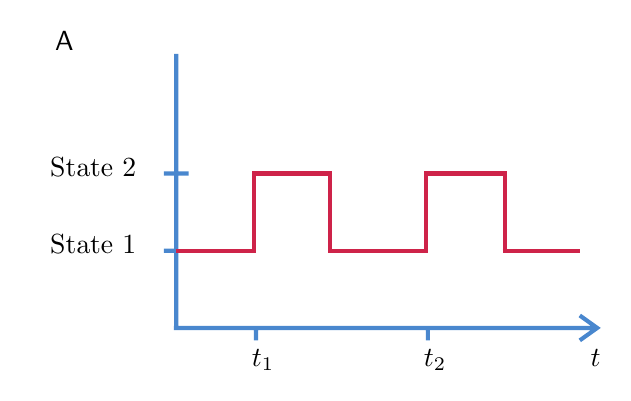
\begin{tikzpicture}[x=0.9pt,y=0.9pt,yscale=-1,xscale=1]
        \path (20,200); %set diagram left start at 0, and has height of 200

        \draw [color={rgb, 255:red, 73; green, 135; blue, 206 }, draw opacity=1 ][line width=1.5][-]
        % axes
        (78.67,210.33) -- (248.67,210.33)
        (79.67,100.33) -- (79.67,210.33)

        % arrow
        (241.67,205.33) -- (248.67,210.33) -- (241.67,215.33)
        %(74.67,105.33) -- (79.67,100.33) -- (84.67,105.33)

        % axis ticks
        (111.67, 210.33) -- (111.67, 215.33)
        (180.67, 210.33) -- (180.67, 215.33)
        (74.67,179.33) -- (79.67,179.33)
        (74.67,148.33) -- (84.67,148.33);
        \draw;

        \draw [color={rgb, 255:red, 206; green, 35; blue, 73 }, draw opacity=1 ][line width=1.5][-]

        (79.67,179.33) -- (111.67,179.33)
        (110.85,179) -- (110.85,147.50)
        (111.67,148.33) -- (140.67,148.33)
        (141.49,147.50) -- (141.49,179)
        (140.67,179.33) -- (180.67,179.33)
        
        (179.85,179) -- (179.85,147.50)
        (180.67,148.33) -- (210.67,148.33)
        (211.49,147.50) -- (211.49,179)
        (210.67,179.33) -- (241.67,179.33);
        \draw;

        \draw [-] (30,90) node [anchor=north west][inner sep=0.75pt] [align=left] {\textsf{A}};
        \draw [-] (28,172) node [anchor=north west][inner sep=0.75pt] [align=left] {State 1};
        \draw [-] (28,141) node [anchor=north west][inner sep=0.75pt] [align=left] {State 2};
        \draw [-] (109,218) node [anchor=north west][inner sep=0.75pt] [align=left] {$t_1$};
        \draw [-] (178,218) node [anchor=north west][inner sep=0.75pt] [align=left] {$t_2$};
        \draw [-] (245,218) node [anchor=north west][inner sep=0.75pt] [align=left] {$t$};

    \end{tikzpicture}
    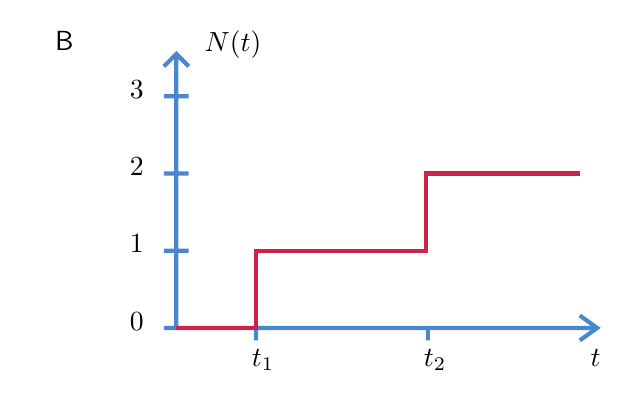
\begin{tikzpicture}[x=0.9pt,y=0.9pt,yscale=-1,xscale=1]
        \path (20,200); %set diagram left start at 0, and has height of 200

        \draw [color={rgb, 255:red, 73; green, 135; blue, 206 }, draw opacity=1 ][line width=1.5][-]
        % axes
        (78.67,210.33) -- (248.67,210.33)
        (79.67,100.33) -- (79.67,210.33)

        % arrow
        (241.67,205.33) -- (248.67,210.33) -- (241.67,215.33)
        (74.67,105.33) -- (79.67,100.33) -- (84.67,105.33)

        % axis ticks
        (111.67, 210.33) -- (111.67, 215.33)
        (180.67, 210.33) -- (180.67, 215.33)

        (74.67,210.33) -- (79.67,210.33)
        (74.67,179.33) -- (84.67,179.33)
        (74.67,148.33) -- (84.67,148.33)
        (74.67,117.33) -- (84.67,117.33);
        \draw;

        \draw [color={rgb, 255:red, 206; green, 35; blue, 73 }, draw opacity=1 ][line width=1.5][-]

        (79.67,210.33) -- (111.67,210.33)
        (111.67,211.15) -- (111.67,178.50)
        (111.67,179.33) -- (180.67,179.33)
        
        (179.85,179) -- (179.85,147.5)
        (180.67,148.33) -- (241.67,148.33);
        \draw;

        \draw [-] (30,90) node [anchor=north west][inner sep=0.75pt] [align=left] {\textsf{B}};
        \draw [-] (60,203) node [anchor=north west][inner sep=0.75pt] [align=left] {0};
        \draw [-] (60,172) node [anchor=north west][inner sep=0.75pt] [align=left] {1};
        \draw [-] (60,141) node [anchor=north west][inner sep=0.75pt] [align=left] {2};
        \draw [-] (60,110) node [anchor=north west][inner sep=0.75pt] [align=left] {3};
        \draw [-] (109,218) node [anchor=north west][inner sep=0.75pt] [align=left] {$t_1$};
        \draw [-] (178,218) node [anchor=north west][inner sep=0.75pt] [align=left] {$t_2$};
        \draw [-] (90,90) node [anchor=north west][inner sep=0.75pt] [align=left] {$N(t)$};
        \draw [-] (245,218) node [anchor=north west][inner sep=0.75pt] [align=left] {$t$};

    \end{tikzpicture}
    \caption[Example of transitions in a multi-state process and the corresponding counting process]{Example of transitions between two states in a multi-state process (panel A), and the corresponding counting process for the State 1 $\rightarrow$ State 2 transition (panel B).}\label{fig:counting-process}
\end{figure}

\subsection{Multi-state models}

In a multi-state model, each state represents a different stage or condition that an individual may experience. The transitions between these states are modelled as a multi-state process, with the time spent in each state and the transitions between states being random variables that can be estimated from data~\parencite{Putter2007-kb}.

Multi-state models are particularly useful in the context of disease progression, as each state in the model can be used to represent a different level of disease severity, with transitions between states representing progression. This may allow for a more nuanced understanding of disease processes, capturing the different pathways that patients may experience~\parencite{Matsena-Zingoni2021-co}.

\subsection{Continuous-time multi-state models}

Continuous-time multi-state models are defined by transition intensities, $q_{r,s}(t, \bm{z}(t))$, which represent the instantaneous hazard of moving from state $r$ to state $s$ at time $t$, dependent on a set of explanatory, potentially time-varying, covariates $\bm{z}(t)$~\parencite{Putter2007-kb}. Defining an individual's state at time $t$ as $X(t)$ then:
%
\begin{equation}
    q_{r,s}(t, \bm{z}(t)) = \lim_{\delta t\downarrow 0}\frac{\Pr(X(t+\delta t)=s \mid X(t)=r)}{\delta t}
    \label{eq:transition-intensity}
\end{equation}

From Equation~\ref{eq:hazard-function}, this transition intensity is equivalent to the hazard of transition from one state to another. These transition intensities form a \textit{transition intensity matrix} $\mathbf{Q}$, whose rows sum to zero, with diagonal entries defined by:
%
\[
    q_{r,r}(t, \bm{z}(t)) = - \sum_{s \neq r} q_{r,s}(t, \bm{z}(t))
\]

For the example three-state model shown in Figure~\ref{fig:basic-msm} this matrix would be:
%
\[
    \mathbf{Q} = \begin{bmatrix}
        -q_{1,2}-q_{1,3} & q_{1,2}          & q_{1,3} \\
        q_{2,1}          & -q_{2,1}-q_{2,3} & q_{2,3} \\
        0                & 0                & 0       \\
    \end{bmatrix}
\]

Here, state 3 is known as an `absorbing' state, as individuals do not leave the state after arrival, while states 1 and 2 are `transient' states. The \textit{transition probability matrix}, which contains the probabilities of moving between states within a time-interval of length $t$ is derived from the transition intensity matrix by the matrix exponential~\parencite{van-den-Hout2016-xy}:
%
\[
    \mathbf{P}(t) = \exp(t\mathbf{Q}) = \sum_{n=0}^{\infty}\frac{t^n}{n!}\mathbf{Q}^n
\]

\subsubsection{Covariates}

The (potentially time-varying) effect of a given set of $m$ covariates, $\bm{z}(t) = \{z_1(t), \ldots, z_m(t)\}$, on the transition intensities $q_{r,s}(t, \bm{z}(t))$ can be expressed via a proportional hazards regression model. Typically these combine a parametric baseline hazard, $q^{(0)}_{r,s}(t)$, with log-linear regression:
%
\begin{align*}
    q_{r,s}(t, \bm{z}(t)) & = q^{(0)}_{r,s}(t)\exp\left(\sum_{m=1}^{M}\beta_{r,s,m}z_{m}(t)\right)  \\
                          & = q^{(0)}_{r,s}(t)\exp\left(\bm{\beta}_{r,s}^\mathsf{T}\bm{z}(t)\right)
\end{align*}

where $\exp(\beta_{r,s,m})$ is the hazard ratio for the $m$th covariate on the $r \rightarrow s$ transition~\parencite{van-den-Hout2016-xy}.

\subsubsection{Sojourn time}

The time spent in a state prior to transition is termed the \textit{sojourn time}, with its mean given by the inverse of the transition intensity for remaining in the state~\parencite{Jackson2011-ry}:
%
\[
    E(T_r) = -\frac{1}{q_{r,r}}
\]

\subsection{Discrete-time multi-state models}

For population studies which measure duration in discrete time, discrete-time multi-state models may applied~\parencite{Steele2004-ru}. Since the concept of instantaneous risk does not apply in discrete time, transition probabilities are instead defined which represent the probability of transition from state $r$ to state $s$ in the time interval $(t_i,t_j]$, $t_j>t_i$:
%
\[
    p_{r,s}(t_i, t_j) = \Pr(X(t_j) = s \mid X(t_i) = r)
\]

\subsection{Semi-Markov and hidden Markov models}

Multi-state models are typically specified to be Markov, i.e.\ $q_{r,s}(t; \mathcal{X}_t) = q_{r,s}(t)$, where $\mathcal{X}_t$ is the observation history of the process up to time $t$. Semi-Markov models relax the Markov assumption, allowing dependence on the time of entry into the current state, i.e.\ $q_{r,s}(t;\mathcal{X}_t)=q_{r,s}(t-t_r)$, where $t_r$ is the time of entry into the current state $r$~\parencite{Meira-Machado2009-xu}.

Hidden Markov models may also be specified to allow for unobserved, or `latent', states to be included in the model. These can be particularly useful for modelling complex disease processes, where progression of the disease is influenced by unobserved factors, and the time to event depends on the current state of the disease, for instance in models of HIV progression~\parencite{Aalen1997-jh}.

\section{Statistical inference for multi-state models}

The non-parametric Aalen-Johansen estimator, parametric multi-state mixture models, and parametric multi-state cause-specific hazards models were demonstrated to provide comparable estimates of competing risks when applied to real-world hospital admissions data~\parencite{Jackson2022-lt}. Mixture models have the advantage that easily interpretable quantities, such as event probabilities and times to events, are directly estimated~\parencite{Andersen2002-ps}. Whereas, for cause-specific hazards models, intensive simulation is required to derive these quantities from parameter estimates that are not directly interpretable~\parencite{Larson1985-ca}. % more information about the difference in these models?

This section describes statistical inference for non-parametric and parametric multi-state survival models. I discuss how these multi-state methods are well-suited to the investigation of intermittently-observed data and explain how these models have been implemented during my PhD.

\subsection{Aalen-Johansen estimator}

The non-parametric Aalen-Johansen estimator can be used to estimate the transition probability matrix, $\mathbf{P}(t)$ for a Markov process with a finite number of states~\parencite{Andersen1996-xs}. Firstly, let $\mathbf{A}(t)$ be the matrix of cumulative transition intensities from state $r$ to state $s$:
%
\[
    \mathbf{A}(t) = A_{r,s}(t) =
    \begin{dcases*}
        \int_{0}^{t}{q_{r,s}(u) \dif u} & if $r\neq s$ \\
        -\sum_{r \neq s}{A_{r,s}(t)}    & if $r = s$
    \end{dcases*}
\]

The transition probability matrix for this process can be represented as:
%
\[
    \mathbf{P} = \prod_{k = 1}^{K}{\left(\mathds{I}+\Delta\mathbf{A}(t_k)\right)}
\]

where $\mathds{I}$ is the identity matrix, $\Delta\mathbf{A}(t_k) = \mathbf{A}(t_k) - \mathbf{A}(t_k \mbox{-})$, and $t_k \mbox{-}$ represents the instant before time $t_k$~\parencite{Andersen1996-xs}. Substituting the Nelson-Aalen estimator for $\mathbf{A}(t)$, then the Aalen-Johansen estimate of the transition probability matrix is:
%
\[
    \mathbf{{\hat{P}}}(t) = \hat{P}_{r,s}(t) = \prod_{k = 1}^{K}{\left(\mathds{I}_{r,s}+\Delta\hat{A}_{r,s}(t_k)\right)}
\]

with:
%
\[
    \Delta\hat{A}_{r,s}(t_k) =
    \begin{dcases*}
        \frac{\Delta N_{r,s}(t_k)}{Y_{r}(t_k \mbox{-})} & if $r\neq s$ \\
        \frac{-\Delta N_{s}(t_k)}{Y_{s}(t_k \mbox{-})}  & if $r = s$
    \end{dcases*}
\]

where $\Delta N_{r,s}(t_k)$ is the number of transitions from state $r$ to state $s$ at time $t_k$, $\Delta N_{s}(t_k)$ is the number of transitions away from state $s$ at time $t_k$, and $Y_{r}(t_k \mbox{-})$ is the number of individuals in state $r$ just before time $t_k$~\parencite{Borgan2014-dv}.

\subsection{Multi-state mixture models}

For a general multi-state competing risks mixture model, assume that an individual $i$ who begins in state $r$ makes a transition to a (pre-assigned) destination state $s$. Let $I_{i,r}$ be the indicator variable which determines which transition will occur, the transition intensity at time $t$ is:
%
\[
    q_{i,r,s}(t) =
    \begin{dcases*}
        q^{*}_{i,r,s}(t) & if $I_{i,r} = s$ \\
        0                & otherwise
    \end{dcases*}
\]

where $q^{*}_{i,r,s}(t)$ is the transition intensity for the transition which occurs. The probability of transition to state $s$ is defined as:
%
\begin{align*}
    \pi_{r,s} & = \Pr(I_{i,r} = s)
\end{align*}

Let $T_{r,s}$ be the the time from entering state $r$ to moving to state $s$, given that this transition occurs (i.e.\ the conditional sojourn time). A parametric distribution with parameters $\theta_{r,s}$ and conditional density $f_{r,s}(. \mid \theta_{r,s})$ may be used to model $T_{r,s}$~\parencite{Ghani2005-or}.

The probabilities of competing events $\pi_{r,s}$ can be related to a set of $m$ covariates $\bm{z} = \{z_1, \ldots, z_m\}$ via multinomial logistic regression. Define as $S_r$ the set of all competing states after $r$, then the logit of transition to a given state $j \in S_r$ vs.\ transition to a baseline state $0 \in S_r$ is:
%
\[
    \ln\left(\frac{\pi_{r,j}(\bm{z})}{\pi_{r,0}(\bm{z})}\right) = \alpha_{r,j} + \bm{\beta}_{r,j}^\mathsf{T} \bm{z}
\]

with $\alpha_{r,j}$ and $\bm{\beta}_{r,j} = \{\beta_{r,j,k};\; k = 1, \ldots m\}$ being regression coefficients for the probability of transition to state $j$~\parencite{Fagerland2008-nb}.

Meanwhile, parameters $\theta_{r,s}$ of the time to transition distribution can be related to a different (or identical) set of $l$ covariates $\bm{z} = \{z_1, \ldots, z_l\}$ via a log-linear model with coefficients $\gamma_{r,s}$ and $\bm{\omega}_{r,s} = \{\omega_{r,s,k};\; k = 1, \ldots, l\}$:
%
\[
    \log(\theta_{r,s}(\bm{z}))=\gamma_{r,s} + \bm{\omega}_{r,s}^\mathsf{T} \bm{z}
\]

For most parametric time to transition distributions `accelerated failure time' models are considered, where the covariates affect the rate of progression of time, i.e.\ the survival function $S(t \mid \bm{z})$ for an individual at time $t$ with covariates $\bm{z}$ is related to the baseline survival $S^{(0)}$ via:
%
\[
    S(t\mid \bm{z}) = S^{(0)}\left(\exp(\bm{\theta}^\mathsf{T}\bm{z})t\right)
\]

where $\bm{\theta}$ is a vector of regression coefficients~\parencite{Klein2005-ls}.

% The likelihood contributions are defined in more detail in the chapter, but kept here for reference

% \begin{itemize}
%     \item for an individual who reaches state $s$ at time $t$:
%           %
%           \[
%               l_i = \pi_i f(t\mid i=s)
%           \]

%     \item for an individual who does not reach a state (e.g.\ remains in hospital) at time $t$:
%           %
%           \[
%               l_c = \sum_{i=1}^k\pi_i(1-F(t\mid i))
%           \]
%           where $F(t\mid i) = \int_0^t f(x\mid i)dx$ is the conditional cumulative distribution.
% \end{itemize}

\subsection{Accounting for censoring}\label{sec:censoring-intermittent}

As described in Section~\ref{sec:likelihood}, survival models may be specified to account for censoring and truncation in observed data by careful consideration and construction of the likelihood function. Multi-state survival models, in particular, are well-suited to investigating interval-censored, or \textit{intermittently-observed} data~\parencite{van-den-Hout2016-xy}.

In Figure~\ref{fig:intermittent-data}, changes in an underlying process were detected with an intermittent observation scheme. Depending on the nature of the underlying process, less frequent and/or irregular observation of the underlying process may result in transitions being undetected, as shown in Figure~\ref{fig:intermittent-missing}.

\begin{figure}[htbp!]
    \centering
    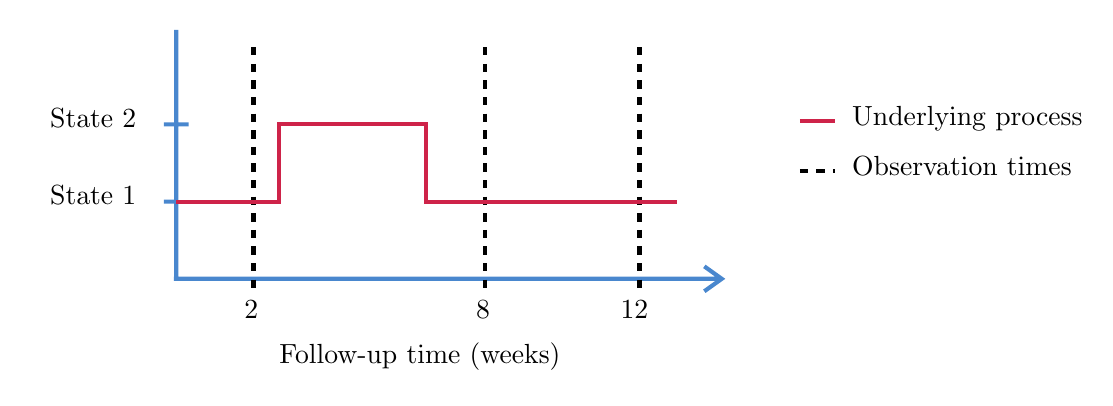
\begin{tikzpicture}[x=0.9pt,y=0.9pt,yscale=-1,xscale=1]
        \path (20,250); %set diagram left start at 0, and has height of 200

        %Shape: Axis 2D [id:dp048941842347560494] 
        \draw [color={rgb, 255:red, 73; green, 135; blue, 206 }, draw opacity=1 ][line width=1.5][-]
        % axes
        (78.67,210.33) -- (298.67,210.33)
        (79.67,110.33) -- (79.67,210.33)

        % arrow
        (291.67,205.33) -- (298.67,210.33) -- (291.67,215.33)

        % axis ticks
        (74.67,179.33) -- (79.67,179.33)
        (74.67,148.33) -- (84.67,148.33);
        \draw;

        \draw [color={rgb, 255:red, 0; green, 0; blue, 0 }, draw opacity=1][line width=1.5][-][dashed]
        (110.67,117.33) -- (110.67,214.33)
        %(141.67,117.33) -- (141.67,214.33)
        %(172.67,117.33) -- (172.67,214.33)
        (203.67,117.33) -- (203.67,214.33)
        %(234.67,117.33) -- (234.67,214.33)
        (265.67,117.33) -- (265.67,214.33)
        (330, 167) -- (344, 167);
        \draw;

        \draw [color={rgb, 255:red, 206; green, 35; blue, 73 }, draw opacity=1 ][line width=1.5][-]

        (79.67,179.33) -- (121.67,179.33)
        (120.85,179) -- (120.85,147.5)
        (120.67,148.33) -- (180.67,148.33)
        (179.85,148.5) -- (179.85,180.15)
        (180.67,179.33) -- (280.67,179.33)
        (330, 147) -- (344, 147);
        \draw;

        %\draw [-] (0,100) node [anchor=north west][inner sep=0.75pt] [align=left] {\textsf{B}};
        \draw [-] (28,172) node [anchor=north west][inner sep=0.75pt] [align=left] {State 1};
        \draw [-] (28,141) node [anchor=north west][inner sep=0.75pt] [align=left] {State 2};
        \draw [-] (106,218) node [anchor=north west][inner sep=0.75pt] [align=left] {2};
        %\draw [-] (137,218) node [anchor=north west][inner sep=0.75pt] [align=left] {4};
        %\draw [-] (168,218) node [anchor=north west][inner sep=0.75pt] [align=left] {6};
        \draw [-] (199,218) node [anchor=north west][inner sep=0.75pt] [align=left] {8};
        %\draw [-] (226,218) node [anchor=north west][inner sep=0.75pt] [align=left] {10};
        \draw [-] (257,218) node [anchor=north west][inner sep=0.75pt] [align=left] {12};
        \draw [-] (120,235) node [anchor=north west][inner sep=0.75pt] [align=left] {Follow-up time (weeks)};

        \draw [-] (350,140) node [anchor=north west][inner sep=0.75pt] [align=left] {Underlying process};
        \draw [-] (350,160) node [anchor=north west][inner sep=0.75pt] [align=left] {Observation times};

    \end{tikzpicture}
    \caption[Example of intermittently-observed data with missed observations for an underlying process]{Example of intermittently-observed data with missed observations for an underlying process.}\label{fig:intermittent-missing}
\end{figure}

An observation scheme is said to be \textit{non-informative} if the likelihood is proportional to a scenario where observation times were fixed in advance and chosen independently of the underlying process~\parencite{Gruger1991-pe}. With a non-informative observation scheme then multi-state models can correctly account for intermittently-observed data~\parencite{van-den-Hout2016-xy}.

\subsection{Implementing multi-state models}

A number of sophisticated statistical software packages exist to implement frequentist and Bayesian survival and multi-state models using the \texttt{R} programming language~\parencite{R_Core_Team2020-ca}. Frequentist maximum likelihood estimation tends to be less computationally intensive than Bayesian inference, and the latter may require integrating over a vast number of parameters, which is usually impracticable for higher dimensions. Instead, algorithms which simulate from the posterior distribution are often used to evaluate features of these integrals. Markov Chain Monte Carlo (MCMC) algorithms have been widely used for this application~\parencite{Young2005-vx}.

The specialised modelling packages used during my PhD have included:\ \texttt{survival}, \texttt{msm} and \texttt{flexsurv} which fit models using maximum likelihood~\parencite{Therneau1999-to, Jackson2011-ry, Jackson2016-tv}, and \texttt{JAGS} and \texttt{STAN}~\parencite{Plummer2003-yj, Carpenter2017-wk} which fit Bayesian models using MCMC\@.

In the spirit of open research, a repository containing code samples for implementing the multi-state methods used during my PhD, and the \texttt{R} code used to generate the figures and tables for this thesis is available at:~\url{https://github.com/pkirwan/PhD-thesis}.

\section{Key concepts in causal inference}\label{sec:causal-inference}

In this final section I introduce the concept of causal inference from observational data and provide an outline of three common methods to compute the average causal effect.

Ideal randomised experiments, where the treated and untreated are exchangeable (or `exogenous'), provide a rigorous way to assess causal effects in a population, as any association between between the treatment and the outcome can be regarded as causation. Whilst this is generally not true for observational data, if an explicit causal question is defined (e.g.\ the effect of a well-specified hypothetical intervention), and certain conditions fulfilled, the same assessment of causation can be made from observational data~\parencite{Hernan2006-ei}.

\subsection{Causal diagrams and local independence}

Causal diagrams are a graphical tool used to visualise causal relationships~\parencite{Aalen2016-to}. One class of causal diagrams are causal directed acyclic graphs (causal DAGs)\nomenclature[z]{DAG}{Directed acyclic graph}. In these graphs, nodes represent measurements or interventions at discrete times, and edges between nodes indicate causal effects, an example is shown in Figure~\ref{fig:causal-dag}. For causal DAGs, the lack of an edge between nodes can be interpreted as the absence of a direct effect~\parencite{Hernan2023-de}.

\begin{figure}[htbp!]
    \centering
    \begin{tikzpicture}
        % x node set with absolute coordinates
        \node (a) at (0,0) {$A$};
        \node (b) [above =of a] {$C$};
        \node (c) [right =of a] {$Y$};
        % Directed edge
        \path (b) edge (a);
        \path (a) edge (c);
        \path (b) edge (c);
    \end{tikzpicture}
    \caption[Example of a causal DAG]{Example of a causal DAG representing discrete measurements for treatment, $A$, causes of treatment, $C$, and outcome, $Y$.}\label{fig:causal-dag}
\end{figure}

Whilst causal DAGs are useful to describe relationships between discrete-time processes, they are poorly suited to describing causality in continuous-time as changes in quantities or the occurrence of events are not represented~\parencite{Aalen2016-to}. Instead, for continuous-time processes, the concept of \textit{local independence} may be applied to consider how well a future value of an intensity process (such as a transition intensity in a multi-state model) is predicted by the past~\parencite{Didelez2008-mq}. Local independence can be viewed as `immediate causation', and can be represented in causal diagrams known as a local independence graph. In these graphs, nodes represent stochastic processes and edges between nodes represent immediate causal influence~\parencite{Aalen2016-to}, as shown in Figure~\ref{fig:local-independence-graph}.

\begin{figure}[htbp!]
    \centering
    \begin{tikzpicture}
    
        % x node set with absolute coordinates
        \node (a) at (0,0) {$A$};
        \node (b) [above =of a] {$C$};
        \node (c) [right =of a] {$Y$};

        % Directed edge
        \path (b) edge[bend right = 10] (a);
        \path (a) edge[bend right = 10] (c);
        %\path (b) edge[bend right = 20] (c);

    \end{tikzpicture}
    \caption[Example of a local independence graph]{Example of a local independence graph representing continuous processes for treatment, $A$, causes of treatment, $C$, and outcome, $Y$. In local independence graphs only immediate causal influences are shown.}\label{fig:local-independence-graph}
\end{figure}

\subsection{Causal inference from observational data}

To make causal inference from observational data we rely on being able to analyse the data as if treatment had been randomly assigned, conditional on a set of measured covariates $Z$. This is termed a `conditionally randomised' experiment~\parencite{Hernan2023-de}.

Let $Y = (0: \text{doesn't experience outcome, } 1: \text{experiences outcome})$ be a random variable for an observed outcome, and $A = (0: \text{untreated, } 1: \text{treated})$ be a random variable for an observed treatment, then:
%
\[
    \Pr(Y = 1 \mid A = 1)
\]

is the probability of experiencing the outcome given treatment. Define the potential outcome under treatment $a$ as $Y^a$, then the potential outcome under the observed treatment:
%
\[
    Y^A = Y
\]

The three `identifiability' conditions required for an observational study to be treated as a conditionally randomised experiment are~\parencite{Hernan2023-de}:
%
\begin{enumerate}
    \item \textbf{Consistency}:\ the values of treatment under comparison correspond to well-defined interventions that, in turn, correspond to the versions of treatment in the data, i.e.
          %
          \[
              Y^a = Y \text{ for individuals with } A = a
          \]

    \item \textbf{Exchangeability}:\ the conditional probability of receiving every value of treatment depends only on measured covariates $Z$. This is alternatively phrased as: conditional on a set of measured covariates $Z$, the untreated group, had they been treated, would experience the same average outcome as the treated group, i.e.
          %
          \[
              \Pr(Y^a = 1 \mid A = 1, Z = z) = \Pr(Y^a = 1 \mid A = 0, Z = z)
          \]

          or equivalently, $Y^a \ind A \mid Z = z$, the counterfactual outcome and the observed treatment are independent within the covariate levels $Z = z$;

    \item \textbf{Positivity}:\ the probability of receiving every value of treatment $a$ conditional on $Z = z$ is positive.
          %
          \[
              \Pr(A = a \mid Z = z) > 0 \quad\text{for all } z \text{ where } \Pr(Z = z) \neq 0
          \]

\end{enumerate}

Among these conditions, consistency and positivity are usually straightforward to check in observational studies whilst exchangeability relies on the assumption that all predictors of an outcome have been measured. It is usually impossible to guarantee exchangeability, but understanding the potential for biases such as confounding and collider bias (defined below) can inform which covariates to include such that the assumption will be approximately true~\parencite{Hernan2023-de}.

If the three identifiability conditions are fulfilled, a (hypothetical) randomised experiment, known as a `target trial', may be emulated using causal inference from observational data, with the average causal effect quantified as $E(Y^{a = 1}) - E(Y^{a = 0})$~\parencite{Hernan2016-be}.

\subsection{Methods to compute the average causal effect}

Three commonly-used methods to compute the average causal effect are inverse probability weighting, matching, and standardisation.

The concept of \textbf{inverse probability weighting} is to assign weights to each individual in the cohort based on the inverse of the probability of receiving the observed treatment level, and conditional on their covariates, $Z$. For example, a treated individual, $A = 1$, with a set of covariates $Z = z$ would be assigned a weight of $1/\Pr(A = 1 \mid Z = z)$. Conversely, an untreated individual, $A = 0$, with covariates $Z = z'$ would be assigned a weight of $1/\Pr(A = 0 \mid Z = z')$. These weights are used to adjust for potential baseline confounders when estimating the causal effect of treatment, allowing the creation of a `pseudo-population' where treatment assignment is independent of the observed covariates~\parencite{Hernan2016-be}.

\textbf{Matching} involves constructing a subset of the population in which the distribution of covariates, $Z$, is the same for the treated and untreated groups. This is typically achieved by pairing each treated individual with an untreated individual with the same or similar covariate values. The causal effect can be estimated as the average difference in outcomes among the matched pairs~\parencite{Hernan2023-de}.

\textbf{Standardisation} involves estimating the counterfactual risk using a weighted average of the risks (or standardisation of the risks) in each covariate level. For example, for a covariate $Z$ with two levels $(0,1)$:
%
\[
    \Pr(Y^a = 1) = \Pr(Y = 1 \mid Z = 1, A = a)\Pr(Z = 1) + \Pr(Y = 1 \mid Z = 0, A = a)\Pr(Z = 0)
\]

which generalises to:
%
\[
    \Pr(Y^a = 1) = \sum_z{\Pr(Y = 1 \mid Z = z, A = a)\Pr(Z = z)}
\]

The standardised mean $E(Y^a) = \sum_z{E(Y \mid Z = z, A = a)\Pr(Z = z)}$ is known as the \textbf{g-formula}~\parencite{Hernan2016-be, Naimi2017-hd}.

\section{Study designs and biases}

In this final section of the chapter I describe a number of observational study designs and several potential sources of bias common to these studies.

Observational studies are common in epidemiology and a valuable resource for understanding infectious disease burden. Several different types of observational study design exist, which may be more or less suitable depending on the research question, the need to control for specific biases, and the feasibility of data collection~\parencite{Baker2023-me}.

\subsection{Observational study designs}

Table~\ref{tab:2x2-table} shows a $2 \times 2$ table which may be used to group participants in observational studies and to inform the calculation of standard statistical measures.

\begin{table}[!h]
    \centering\centering
    \caption{\label{tab:2x2-table}A $2 \times 2$ table of outcomes and exposures.}
    \centering
    \begin{tabular}{@{}cc|cc@{}}
                                                  &     & \multicolumn{2}{l}{Outcome}       \\ \midrule
                                                  &     & Yes                         & No  \\ \midrule
        \multirow{2}{*}{\rotatebox{90}{Exposure}} & Yes & $A$                         & $B$ \\[3.5ex]
                                                  & No  & $C$                         & $D$
    \end{tabular}
\end{table}

\subsubsection{Cross-sectional studies}

Cross-sectional studies may be used to assess the prevalence of an outcome, defined as:\ $(A+C)/(A+B+C+D)$, and the prevalence of various different exposures, defined as:\ $(A+B)/(A+B+C+D)$, within a population. They provide a snapshot of the population at a single point in time and can be relatively straightforward to conduct using surveillance data~\parencite{Baker2023-me}.

\subsubsection{Case-control studies}

Case-control studies are used to investigate the effects of specific exposures on an outcome. In these studies the outcome of interest has already occurred, individuals who have experienced the outcome are termed `cases', and are compared to individuals without the outcome, known as `controls'. The odds of being exposed are compared in cases vs.\ controls via the odds ratio, defined as:\ $AD/BC$~\parencite{Woodward2013-ef}.

\subsubsection{Test-negative case-control studies}

Test-negative case-control studies are a sub-type of case-control study. These studies aim to minimise bias specifically as a result of test-seeking behaviour by selecting only individuals who test for a disease. As for case-control studies, the cases are individuals who test positive, controls are those who test negative, and again the odds of being exposed are compared between cases and controls.

\subsubsection{Cohort studies}

In cohort studies participants are selected based on their exposure status and followed up over time. The incidence of the outcome of interest is compared between individuals with and without the exposure using the relative risk~\parencite{Woodward2013-ef}:
%
\[
    \frac{A/(A+B)}{C/(C+D)}
\]

For further discussion of test-negative case-control and cohort study designs, see Section~\ref{sec:cohort-study-design}.

\subsection{Biases in observational studies}\label{sec:observational-bias}

Bias can be defined as ``any process at any stage of inference which tends to produce results or conclusions that differ systematically from the truth''~\parencite{Sackett1979-xy}. All of the observational study designs described can include potential sources of bias, which are often grouped into three broad types:\ information bias, collider bias, and confounding~\parencite{Hernan2023-de}.

\subsubsection{Information bias}

Information, or measurement, bias arises due to inaccuracies in data and may be induced by errors or missing information in either the outcome or exposure variables, for example, incorrect coding of a diagnosis~\parencite{Hernan2023-de}. Information bias can be mitigated through careful study design and data collection mechanisms, these could include:\ double entry of data, and linking information across different systems for validation~\parencite{Page2008-on}.

\subsubsection{Collider bias}

Collier bias, or selection bias, occurs when individuals are selected into an analysis by conditioning on a common `collider' variable (a variable which is influenced by two other variables). Figure~\ref{fig:collider-bias} shows an example of collider bias:\ people who are regular smokers and people at high risk of severe COVID-19 illness are both more likely to be admitted to hospital. By conditioning on hospitalisation a distorted association between smoking and COVID-19 mortality could be induced, and this bias may occur in either a positive or negative direction\footnote{A negative association between smoking and COVID-19 severity was reported by more than one early risk-factor study for COVID-19, with a review concluding this result may have been a result of collider bias~\parencite{Wenzl2020-fo}.}.

Collider bias is most easily avoided by not conditioning on the collider, but this may be impractical depending on the nature of data collection~\parencite{Holmberg2022-hb}. In the context of COVID-19,~\cite{Griffith2020-il} have suggested several methods for assessing the sensitivity of model results to collider bias, such as inverse probability weighting. Where information is available, the extent of the bias can also be examined by comparing the profile of selected individuals to the wider population of interest, e.g.\ whether hospitalised individuals tend to be older or more likely to have comorbidities.

\begin{figure}[htbp!]
    \centering
    \begin{tikzpicture}
        \path (0.4,0.4);
        \path (-2.5,-2.5);
        % Nodes
        \node[state, align=center, minimum width = 22mm] (c) at (0,0) {Hospitalisation};
        \node[state, align=center, minimum width = 22mm] (e) [below left = 10mm and -2mm of c] {Regular\\smoker};
        \node[state, align=center, minimum width = 22mm] (o) [right = 25mm of e] {COVID-19\\severity};
        % Edges
        \path (e) edge (c);
        \path (o) edge (c);
        \path[dashed, -] (e) edge (o);
    \end{tikzpicture}
    \caption[Causal diagram showing the effect of collider bias]{Causal diagram showing the effect of collider bias, where conditioning on hospitalisation induces a distorted association between smoking and COVID-19 severity. Conditioned on variables have bounding boxes, distorted associations are shown as dashed lines.}\label{fig:collider-bias}
\end{figure}

\subsubsection{Confounding}

Confounding is related to collider bias, but occurs by not conditioning on an explanatory variable. As a result confounding is sometimes termed `latent variable' bias. Confounding introduces a `backdoor path', an additional source of association between the explanatory variable and the outcome, so the association cannot be interpreted as a causal effect~\parencite{Hernan2023-de}.

An example of confounding is shown in the causal diagram in Figure~\ref{fig:confounding}:\ during vaccine roll-out older people were more likely to receive a COVID-19 vaccine, but also more likely to experience severe COVID-19. If age group is not adjusted for then a distorted association between vaccination and COVID-19 severity may be induced. Confounding can be avoided by ensuring that factors that might be associated with the outcome are measured and adjusted for~\parencite{Hernan2023-de}.

\begin{figure}[htbp!]
    \centering
    \begin{tikzpicture}
        % Nodes
        \node[align=center, minimum width = 22mm] (c) at (0,0) {Age group};
        \node[state, align=center, minimum width = 22mm] (o) [below right = 10mm and -2mm of c] {COVID-19\\severity};
        \node[state, align=center, minimum width = 22mm] (e) [left = 20mm of o] {Vaccination};
        % Edges
        \path (c) edge (e);
        \path (c) edge (o);
        \path[dashed, -] (e) edge (o);

    \end{tikzpicture}
    \caption[Causal diagram showing the effect of confounding]{Causal diagram showing the effect of confounding, where not conditioning on age group induces a distorted association between vaccination and COVID-19 severity. Conditioned on variables have bounding boxes, distorted associations are shown as dashed lines.}\label{fig:confounding}
\end{figure}

\subsubsection{Epidemic phase bias}

Epidemic phase bias occurs in studies with time-varying incidence of infection. This bias is induced by a relationship between the time from infection to symptom onset and an individual's eventual outcome, e.g.\ those who go on to die may experience a more rapid onset of symptoms following infection, an average of $c$ days sooner. Since estimates must be conditioned on the observed symptom onset date, rather than the unobserved infection date, this relationship can introduce bias into results when an epidemic is in a mode of growth or decline~\parencite{Seaman2022-tl}.

Epidemic phase bias is corrected by `shifting' the symptom onset date among those who experience the more severe outcome to be $c$ days later, so that the time from infection to symptom onset is uncorrelated with the outcome (the time-to-event of interest remains the same for both outcomes.) As the true value of $c$ is typically unknown, sensitivity analysis with differing values of $c$ can be used to assess the susceptibility of results to this bias~\parencite{Seaman2022-tl}.